%%%%%%%%%%%%%%%%%%%%%%%%%%%%%%%%%
%
%       EXERCÍCIO
%
%%%%%%%%%%%%%%%%%%%%%%%%%%%%%%%%%

\ifdefstring{\atividade}{prova}{%
    \ifdefstring{\modo}{objetivo}{%
        \renewcommand{\valorquestao}{\ValorQObj\ ponto}
    }{%
        \renewcommand{\valorquestao}{\ValorQDisc\ pontos}
    }%
}%

\begin{exercicioBanco}[\valorquestao]
Considere a função \(f:[-3,6] \to [-3,3]\), cujo gráfico está abaixo.
%
\begin{center}
    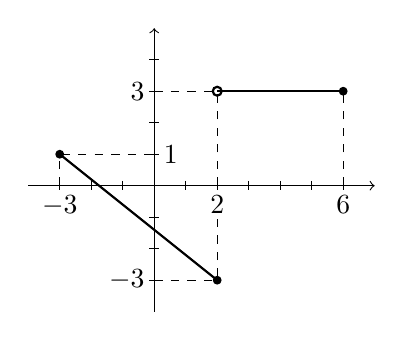
\begin{tikzpicture}[scale=0.4]

    % Eixos
    \draw[->] (-4,0) -- (7,0);      % eixo x
    \draw[->] (0,-4) -- (0,5);      % eixo y

    % Marcas principais
    \foreach \x in {-3,-2,-1,1,2,3,4,5,6}
        \draw (\x,0.15) -- (\x,-0.15);

    \foreach \y in {-3,-2,-1,1,2,3,4}
        \draw (0.15,\y) -- (-0.15,\y);

    % Rótulos importantes
    \node[below] at (-3,0) {$-3$};
    \node[below] at (2,0) {$2$};
    \node[right] at (0,1) {$1$};
    \node[below] at (6,0) {$6$};
    \node[left] at (0,3) {$3$};
    \node[left] at (0,-3) {$-3$};

    % Segmento inclinado
    \draw[thick] (-3,1) -- (2,-3);

    % Pontos fechados do segmento inclinado
    \fill (-3,1) circle (4pt);
    \fill (2,-3) circle (4pt);

    % Segmento horizontal superior
    \draw[thick] (2,3) -- (6,3);

    % Círculo aberto em (2,3)
    \draw[thick] (2,3) circle (4pt);

    % Ponto fechado em (6,3)
    \fill (6,3) circle (4pt);

    % Linhas tracejadas auxiliares
    \draw[dashed] (2,0) -- (2,3);
    \draw[dashed] (6,0) -- (6,3);
    \draw[dashed] (0,3) -- (2,3);
    \draw[dashed] (0,-3) -- (2,-3) -- (2,-1);
    \draw[dashed] (-3,0) -- (-3,1) -- (0,1);

    \end{tikzpicture}
\end{center}
%
Determine o valor de \(\dfrac{f(5)}{f(-3)-f(2)}\).

% Define as alternativas
\newcommand{\alternativas}{%
    \begin{center}
        \begin{tabularx}{\textwidth}{XXXXX}
            (a) \(\dfrac{1}{4}\). &
            (b) \(\dfrac{2}{4}\). &
            (c) \(\dfrac{3}{4}\). &
            (d) \(1\). &
            (e) \(\dfrac{5}{4}\).
        \end{tabularx}
    \end{center}
}

% Define a resposta correta
\newcommand{\resposta}{C}

% Lógica condicional para exibição
\ifdefstring{\atividade}{lista}{%
    \alternativas
    \vspace{0.5em}
    
    \noindent\textbf{Resposta:} letra \textbf{\resposta}.
}{%
    \ifdefstring{\modo}{objetivo}{%
        \alternativas
    }{%
        % modo = discursiva → não mostra alternativas
    }
}
\end{exercicioBanco}

